\documentclass[
a4paper,        			% alle weiteren Papierformat einstellbar
DIV=12,
%landscape,					% Querformat
11pt,						% Schriftgroesse (12pt, 11pt (Standard))
BCOR=10mm,					% Bindekorrektur, bspw. 1 cm
%DIVcalc,				    % fuehrt die Satzspiegelberechnung neu aus s. scrguide 2.4
oneside,					% einseitiges Layout
%twocolumn,				    % zweispaltiger Satz
%openany,					% Kapitel koenen auch auf linken Seiten beginnen
%halfparskip*,				% Absatzformatierung s. scrguide 3.1
%headsepline,				% Trennline zum Seitenkopf	
%footsepline,    			% Trennline zum Seitenfu
%notitlepage,				% in-page-Titel, keine eigene Titelseite
%chapterprefix,				% vor Kapitelueberschrift wird "Kapitel Nummer" gesetzt
%appendixprefix,			% Anhang wird "Anhang" vor die ueerschrift gesetzt
headings = normal,			% ueerschriften etwas kleiner (smallheadings)
%idxtotoc,					% Index im Inhaltsverzeichnis
listof=totoc,				% Abb.- und Tab.verzeichnis im Inhalt
bibliography=totoc,			% Literaturverzeichnis im Inhalt
%leqno				    	% Nummerierung von Gleichungen links
%fleqn,						% Ausgabe von Gleichungen linksbundig
%draft			    		% ueberlangen Zeilen in Ausgabe gekennzeichnet
]
{scrartcl}

%% Include Packages and Settings%%%%%%%%%%%%%%%%%%%%%%%%%%%%%%%%%%%%%%%
\usepackage[utf8]{inputenc}
%see files examples for examples...

%% Set Language %%%%%%%%%%%%%%%%%%%%%%%%%%%%%%%%%%%%%%%%%%%%%%%%%%%%%%%%%%%%%%%
\usepackage[english]{babel}
\usepackage[T1]{fontenc}
%\usepackage[ansinew]{inputenc}

%%\usepackage[ngerman]{babel}
%%\usepackage[T1]{fontenc}
%%\usepackage[ansinew]{inputenc}

%% General Stuff %%%%%%%%%%%%%%%%%%%%%%%%%%%%%%%%%%%%%%%%%%%%%%%%%%%%%%%%

\usepackage{amsmath} % AMS Math Package
\usepackage{amsthm} % Theorem Formatting
\usepackage{amssymb}	% Math symbols such as \mathbb
\usepackage{multicol} % Allows for multiple columns

\usepackage{booktabs} %use \toprule, \bottomrule & \midrule in tables
\usepackage[section]{placeins} %Keep figures within section.
\usepackage{longtable}
\usepackage{array} 

\usepackage{lmodern} %enhanced versions of the Computer Modern fonts
\usepackage{epigraph} %good looking quotes

\usepackage{nicefrac} %nice fractions
\usepackage{units} %setting units in a typographically correct way
\usepackage{upgreek} %upright typesetting for greek symbols (eg. \upmu and \Upmu
\usepackage[version=3]{mhchem} %use of subscripts within the text environment to typeset chemical formulas, use like \ce{H2O}

%\usepackage[draft]{graphicx} %l�dt nur Platzhalter
\usepackage{graphicx} %%Zum Laden von Grafiken
\usepackage{wrapfig} %%Graphics with text wrpping around
\usepackage{subcaption}  %Placing figures/tables side-by-side,
\usepackage{caption}

%\usepackage[backend=bibtex, sorting=none, style=numeric, natbib=true, sortlocale=en_US, url=false, doi=true, eprint=false]{biblatex}
%\addbibresource{tex/bibo.bib}

\usepackage{csquotes} %%Context sensitive quotation facilities

\usepackage{url}	%creates clickable urls by entering \url{http://www.url.de}
%\usepackage{doi}	%hy­per­link to the tar­get of the DOI.

\usepackage[dvips,a4paper,margin=0.75in,bottom=1 in]{geometry}

%\usepackage{paralist} % very flexible & customisable lists (eg. enumerate/itemize, etc.)
%\usepackage{subcaption} 
%\usepackage[lofdepth,lotdepth]{subfig}include the subs in the listoffigures and listoftables
%\usepackage[cmyk]{xcolor} %convert all to CMYK

%% General Page Layout %%%%%%%%%%%%%%%%%%%%%%%%%%%%%%%%%%%%%%%%%%%%%%%%%%%%%%%

%\usepackage[left=20mm,					% linker Seitenrand f�rs Binden
						%right=20mm,					% rechter Seitenrand
						%top=25mm,					%	oberer Rand
						%bottom=25mm,				% unterer Rand
						%footskip=15mm,			% frei f�r Fu�noten
						%lines=34,					% Rumpf Zeilenauslastung
						%]{geometry}	

\usepackage{setspace}	% Zeilenabstand, MUSS vor hyperref kommen!
	%\setstretch{1}		% Gr��e des Zeilenabstandes


%% FROM FA %%%%%%%%%%%%%%%%%%%%%%%%%%%%%%%
\usepackage{expdlist} %erweiter Formationsmöglichkeiten der description Umgebung

%% Header, Fooder, Chapter Headings and such %%%%%%%%%%%%%%%%%%%%%%%%%%%%%%%
\usepackage{fancyhdr}
\fancyhead{}  % Delete current header settings
\fancyfoot{}  % Delete current footer settings         

% pages and right on odd pages
\fancyhead[L]{\nouppercase{\leftmark}}      % Chapter in the right on even pages
%\fancyhead[R]{\nouppercase{\rightmark}}     % Section in the left on odd pages

\fancyfoot[C]{\thepage}  % Page number (boldface) centered everywhere

\renewcommand{\headwidth}{\textwidth} %set header width to text  width

%\usepackage[Lenny]{fncychap} %fancy chapter headings						


%% Bibliographiestil %%%%%%%%%%%%%%%%%%%%%%%%%%%%%%%%%%%%%%%%%%%%%%%%%%%%%%%%%%
%\usepackage[numbers,square,sort&compress]{natbib}


%% Special Tricks %%%%%%%%%%%%%%%%%%%%%%%%%%%%%%%%%%%%%%%%%%%%%%%%%%%%%%%%%%%

% Line break after \paragraph{Paragraph Name}						
\makeatletter
\renewcommand\paragraph{\@startsection{paragraph}{4}{\z@}%
  {-3.25ex\@plus -1ex \@minus -.2ex}%
  {1.5ex \@plus .2ex}%
  {\normalfont\normalsize\bfseries}}
\makeatother

% Kreis um Zahl, use as \myCircle{Zahl} %%%%%%%%%%%%%%%%%%%%%%%%%%%%%%%%%%%%%%
\newcommand{\myCircle}[1]{ \unitlength1ex\begin{picture}(2.5,2.5)%
\put(0.75,0.75){\circle{2.5}}\put(0.75,0.75){\makebox(0,0){#1}}\end{picture}} 

%% Source code printer for LATEX - Code direct in the .tex file %%%%%%%%%%%%%
\usepackage{listings} %highlighting of all the most common languages 
\usepackage{color}
 
\definecolor{dkgreen}{rgb}{0,0.6,0}
\definecolor{gray}{rgb}{0.5,0.5,0.5}
\definecolor{mauve}{rgb}{0.58,0,0.82}
 
\lstset{ %
  language=Mathematica,                % the language of the code
  basicstyle=\footnotesize,           % the size of the fonts that are used for the code
  numbers=left,                   % where to put the line-numbers
  numberstyle=\footnotesize,          % the size of the fonts that are used for the line-numbers
  stepnumber=1,                   % the step between two line-numbers. If it's 1, each line 
                                  % will be numbered
  numbersep=5pt,                  % how far the line-numbers are from the code
  backgroundcolor=\color{white},      % choose the background color. You must add \usepackage{color}
  showspaces=false,               % show spaces adding particular underscores
  showstringspaces=false,         % underline spaces within strings
  showtabs=false,                 % show tabs within strings adding particular underscores
  %frame=single,                   % adds a frame around the code
  tabsize=2,                      % sets default tabsize to 2 spaces
  captionpos=b,                   % sets the caption-position to bottom
  breaklines=true,                % sets automatic line breaking
  breakatwhitespace=false,        % sets if automatic breaks should only happen at whitespace
  title=\lstname,                   % show the filename of files included with \lstinputlisting;
                                  % also try caption instead of title
  numberstyle=\tiny\color{gray},        % line number style
  keywordstyle=\color{blue},          % keyword style
  commentstyle=\color{dkgreen},       % comment style
  stringstyle=\color{mauve},         % string literal style
  escapeinside={\%*}{*)},            % add a comment within your code
  morekeywords={*,ParallelTable, ParallelMap, Blur, ImageResize, ColorConvert, ImageDimensions, ImageData, ImageTake, ErrorListPlot} % if you want to add more keywords to the set
}




% ***********************************************************
% ******************* PHYSICS HEADER ************************
% ***********************************************************

 % Sets margins and page size
\makeatletter % Need for anything that contains an @ command 
\renewcommand{\maketitle} % Redefine maketitle to conserve space
{ \begingroup \vskip 10pt \begin{center} \large {\bf \@title}
	\vskip 10pt \large \@author \hskip 20pt \@date \end{center}
  \vskip 10pt \endgroup \setcounter{footnote}{0} }
\makeatother % End of region containing @ commands
\renewcommand{\labelenumi}{(\alph{enumi})} % Use letters for enumerate
% \DeclareMathOperator{\Sample}{Sample}
\let\vaccent=\v % rename builtin command \v{} to \vaccent{}
\renewcommand{\v}[1]{\ensuremath{\mathbf{#1}}} % for vectors
\newcommand{\gv}[1]{\ensuremath{\mbox{\boldmath$ #1 $}}} 
% for vectors of Greek letters
\newcommand{\uv}[1]{\ensuremath{\mathbf{\hat{#1}}}} % for unit vector
\newcommand{\abs}[1]{\left| #1 \right|} % for absolute value
\newcommand{\avg}[1]{\left< #1 \right>} % for average
\let\underdot=\d % rename builtin command \d{} to \underdot{}
\renewcommand{\d}[2]{\frac{d #1}{d #2}} % for derivatives
\newcommand{\dd}[2]{\frac{d^2 #1}{d #2^2}} % for double derivatives
\newcommand{\pd}[2]{\frac{\partial #1}{\partial #2}} 
% for partial derivatives
\newcommand{\pdd}[2]{\frac{\partial^2 #1}{\partial #2^2}} 
% for double partial derivatives
\newcommand{\pdc}[3]{\left( \frac{\partial #1}{\partial #2}
 \right)_{#3}} % for thermodynamic partial derivatives
\newcommand{\ket}[1]{\left| #1 \right>} % for Dirac bras
\newcommand{\bra}[1]{\left< #1 \right|} % for Dirac kets
\newcommand{\braket}[2]{\left< #1 \vphantom{#2} \right|
 \left. #2 \vphantom{#1} \right>} % for Dirac brackets
\newcommand{\matrixel}[3]{\left< #1 \vphantom{#2#3} \right|
 #2 \left| #3 \vphantom{#1#2} \right>} % for Dirac matrix elements
\newcommand{\grad}[1]{\gv{\nabla} #1} % for gradient
\let\divsymb=\div % rename builtin command \div to \divsymb
\renewcommand{\div}[1]{\gv{\nabla} \cdot #1} % for divergence
\newcommand{\curl}[1]{\gv{\nabla} \times #1} % for curl
\let\baraccent=\= % rename builtin command \= to \baraccent
\renewcommand{\=}[1]{\stackrel{#1}{=}} % for putting numbers above =
\newtheorem{prop}{Proposition}
\newtheorem{thm}{Theorem}[section]
\newtheorem{lem}[thm]{Lemma}
\theoremstyle{definition}
\newtheorem{dfn}{Definition}
\theoremstyle{remark}
\newtheorem*{rmk}{Remark}

% ***********************************************************
% ********************** END HEADER *************************
% ***********************************************************

\usepackage[pdfstartview={FitV},hidelinks]{hyperref} %enables typesetting of followable hyperlinks, leave it HERE! as it NEEDS to be loaded last!

\pagenumbering{alph}

%TitlePage%%%%%%%%%%%%%%%%%%%%%%%%%%%%%%%%%%%%%%%%%%%%%%%%%%%%%%%%%
\begin{document}

\begin{center}
\Large
\textbf{Optical Imaging in Biology and Medicine\\
Master in Photonics \& Europhotonics Master Program\\
\vspace{1em}
\huge 
Adaptive Optics for Microscopy}\\
\vspace{2em}
\Large
Carles Otero Molins\\
Johannes Rebling\\
\vspace{.2em}
\today
\end{center}

\pagestyle{empty}
\numberwithin{equation}{section} % prepend the section number to all equation numbers, only to use with the amsmath package, has to be here for compatibility reasons...don't ask me...

\section*{Abstract}

Lorem ipsum dolor sit amet, qui ei case inani noster, malis tantas expetenda id qui. Vel assum labore intellegat et. Eu vis vero fastidii intellegebat, ea omnis tation definiebas usu. Ea cetero maiorum convenire sed. Wisi impetus aperiri quo at.

Vis tation maiorum facilisis an, quo ei summo pericula consetetur. Illum quodsi euripidis ex est. Duo ea soluta causae sanctus. Eu pro dolorum imperdiet ullamcorper, quas oporteat at pro, ius an appellantur complectitur. Ea nam aperiri fierent invenire, nam in purto illum iracundia, ei facilisi iracundia scribentur ius. Utroque dolores ex est, ius an tation suscipiantur, ne iriure aperiam quaestio mel. Cum enim legere impedit ex, per ut blandit vituperata conclusionemque, ad aliquid vivendum usu.
\newline

%\clearpage

%Inhaltsverzeichnis%%%%%%%%%%%%%%%%%%%%%%%%%%%%%%%%%%%%%%%%%%%%%%%%%%%%%%%%%
%\pagestyle{plain}
%\pagenumbering{Roman}
%\setcounter{page}{1}
 
\tableofcontents
\clearpage

\pagestyle{fancy}      % Sets fancy header and footer
\pagenumbering{arabic}
\setcounter{page}{1}

%The Introduction section clarifies the motivation for the work presented and 
%prepares readers for the structure of the paper.
% context:  orient those readers who are less familiar with your topic and to 
%establish the importance of your work
% need: state the need for your work, as an opposition between what the 
%scientific community currently has and what it wants.
% task: indicate what you have done in an effort to address the need (this is 
%the task)
% object: preview the remainder of the paper to mentally prepare readers for 
%its structure, in the object of the document
%%%%%%%%%%%%%%%%%%%%%%%%%%%%%%%%%%%%%%%%%%%%%%%%%%%%%%%%%%%%%%%%%%%%%%%%%%%%%%%
\section{Introduction}
\label{sec:Introduction}
%%%%%%%%%%%%%%%%%%%%%%%%%%%%%%%%%%%%%%%%%%%%%%%%%%%%%%%%%%%%%%%%%%%%%%%%%%%%%%%

% explain why this is interesting, why it gives us advantages
% also see general comments above, this intro can be quite short, put the 
actual techniques in the second part, methods

%everything that I posted into your part has been just copied from papers, so 
%you should use it as an inspiration, but you have to write your own text. And 
%please remember to cite every work you base your writing on (i put the 
%references in for the stuff that I copied already) 

% I think this paper that we found gives some good ideas for a good introduction!
\cite{AOM_biomedical}

The performance of these microscopes is often compromised by aberrations that lead to a reduction image resolution and contrast. 

These aberrations may arise from imperfections in the optical system or may be introduced by the physical properties of the specimen.
 
The problems caused by aberrations can be overcome using adaptive optics, whereby aberrations are corrected using a dynamic element, such as a deformable mirror.

This technology was originally conceived for the compensation of the aberrating effects of the atmosphere and was first developed for military and astronomical telescopes. 

Adaptive optics systems have also been introduced for other applications such as laser beam shaping, optical communications, data storage, ophthalmology and microscopy.\\

\cite{AOM_basic_ref}

Optical microscopes have long been essential tools in many scientific disciplines, particularly the biological and medical sciences. Conventional widefield microscopes—encompassing transmission, phase contrast and fluorescence imaging modes—are the workhorses of many laboratories. Over the last 25 years, researchers have also made significant developments in 3-D imaging using scanning laser microscopes. This progress started with the confocal microscope, which provides 3-D resolution by using a pinhole to exclude out-of-focus light. Rather than produce a whole image simultaneously, these microscopes scan a laser spot through the specimen, building the image point-by-point. This achievement was followed by several other laser-scanning methods, including the commonly used twophoton fluorescence microscope. Rather than using a pinhole to generate 3-D discrimination, this microscope relies on the nonlinear process of two-photon excitation to ensure that fluorescence is only generated in the focus, where the laser intensity is highest. Various advances in this field have led to improvements in resolution and contrast. Standard laboratory microscopes now regularly produce images revealing 3-D structure on the submicrometer scale. Several new methods of nanoscopy that combine optical and photophysical phenomena can even beat the diffraction limit to resolve details on the tens-of-nanometers scale.
 
These methods all rely on careful engineering to ensure that the optics operate at the diffraction limit, so that optimum resolution and efficiency are achieved. However, one part of the optical system—the specimen—lies outside the design specification. It is optically inhomogeneous and exhibits spatially varying refractive indices. Hence, the light focused into the specimen suffers from wavefront distortions— or phase aberrations—that degrade the resolution and imaging efficiency of the microscope. The aberrations vary from one specimen to another, so they cannot be corrected by a fixed optical design. Dynamic correction is necessary. This is where adaptive optics (AO) comes into play. 

Adaptive optics was originally conceived for use in astronomical telescopes. These AO systems detect aberrations introduced by the atmosphere and use a deformable mirror to remove the aberrations before the light reaches the imaging detector. For imaging systems with small apertures, such as our eyes, the turbulence causes twinkling; for wider telescope apertures, it leads to severe image blurring that limits the resolution of the telescope. 

The AO approach has been widely applied in astronomy, and it has also found application in ophthalmic imaging, laser-based fabrication, optical communications and, of course, microscopy. The adoption of AO for microscopes has brought new challenges that have required innovative solutions.

\cite{AOM_biomedical}

\clearpage

%%%%%%%%%%%%%%%%%%%%%%%%%%%%%%%%%%%%%%%%%%%%%%%%%%%%%%%%%%%%%%%%%%%%%%%%%%%%%%%
\section{Aberration Measurement and Correction}
%%%%%%%%%%%%%%%%%%%%%%%%%%%%%%%%%%%%%%%%%%%%%%%%%%%%%%%%%%%%%%%%%%%%%%%%%%%%%%%

%explain what are abberations, how they arrise, why it is good to correct them
%I just proposed a rough structure, but I am realizing now, that all the 
%sub-sub-section will take up a lot of room. so it might be better if you 
%remove them an explain it all in one subsection
%here is some stuff that I collected/copied from the paper you gave me

For the purpose of understanding the operation of an adaptive optical system, 
it is best to think of aberrations in terms of distortions of an optical 
wavefront.

\begin{figure}[tbh]
        \centering
        \begin{subfigure}[b]{0.4\textwidth}
                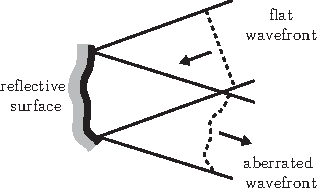
\includegraphics[width=\textwidth]{images/wavefront_distortions_reflection}
                \caption{Reflection.}
                \label{fig:abberation_reflection}
        \end{subfigure}
				\hspace{1em}
        \begin{subfigure}[b]{0.3\textwidth}
                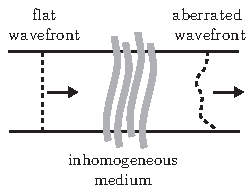
\includegraphics[width=\textwidth]{images/wavefront_distortions_transmission}
                \caption{Transmission.}
                \label{fig:abberation_trans}
        \end{subfigure}
        \caption{Wavefront aberrations due to (a) reflection from a non 
planar surface and (b)  caused by propagation through a non-uniform 
refractive index distribution. Image after~\cite{Aberrations_book}.}
\label{fig:abberations}
\end{figure} 

Representing aberrations in this way can simplify the design, control and 
characterisation of adaptive optics. The choice of modes for a particular 
application is often influenced by some aspect of the system, such as the 
deformation modes of a deformable mirror or the statistics of the induced 
aberrations. Otherwise, the modal representation may be chosen through 
mathematical convenience. For example, Zernike polynomials are often used for 
systems with circular apertures as they form a complete, orthogonal set of 
functions defined over a unit circle

As with all optical systems, microscopes can also suffer from aberrations due 
to imperfections in the optical components. In practice, no system can be 
totally free from aberrations and so systems are designed to maintain 
aberrations below a particular tolerance for a given set of imaging 
conditions, such as wavelength, magnification and field of view. Significant 
aberrations can be introduced if a microscope is used outside its design 
specifications, for example at the incorrect wavelength or at a difierent 
temperature (see Chapter 11 of Ref. 9).

\cite{AOM_basic_ref}


%%%%%%%%%%%%%%%%%%%%%%%%%%%%%%%%%%%%%%%%%%%%%%%%%%%%%%%%%%%%%%%%%%%%%%%%%%%%%%%
\subsection{Wavefront Sensing}
\label{sec:WavefrontSensing}

%------------------------------------------------------------------------------
\subsubsection{Interferometry}
\label{sec:DirectWavefrontSensing_interferometry}
%not sure if this is used for microscopy, we should at least mention it

%------------------------------------------------------------------------------
\subsubsection{Shack-Hartman Wavefront Sensor}
\label{sec:DirectWavefrontSensing_SHWS}

%------------------------------------------------------------------------------
\subsubsection{Indirect Wavefront Sensing}
\label{sec:IndirectWavefrontSensing}

%%%%%%%%%%%%%%%%%%%%%%%%%%%%%%%%%%%%%%%%%%%%%%%%%%%%%%%%%%%%%%%%%%%%%%%%%%%%%%%
\subsection{Aberration Correction}
\label{sec:AberrationCorrection}
% just mention the basic principles, i.e. liquid crystal, deformable mirror, 
computational

%------------------------------------------------------------------------------
\subsection{Deformable Mirror }
\label{sec:DeformableMirror}

%------------------------------------------------------------------------------
\subsubsection{Liquid Crystal Spatial Light Modulators}
\label{sec:LiquidCrystalSpatialLightModulators}
% I used Nematic Liquid Crystalls for my Bachelor Thesis, so if you need 
% infos or graphs about them, let me know and I might be able to help

%%%%%%%%%%%%%%%%%%%%%%%%%%%%%%%%%%%%%%%%%%%%%%%%%%%%%%%%%%%%%%%%%%%%%%%%%%%%%%%
\subsection{Control Strategies}
\label{sec:ControlStrategies}

\clearpage
%The Materials and Methods section provides sufficient detail for other 
%scientists to reproduce the experiments presented in the paper. In some 
%journals, this information is placed in an appendix, because it is not what 
%most readers want to know first.

% explicit preview would be phrased much like the object of the document: 
%"This section first . . . , then . . . , and finally . . . "
% Do not make readers guess: Make sure the paragraph's first sentence gives 
%them a clear idea of what the entire paragraph is about.
%%%%%%%%%%%%%%%%%%%%%%%%%%%%%%%%%%%%%%%%%%%%%%%%%%%%%%%%%%%%%%%%%%%%%%%%%%%%%%
\section{Adaptive Optics Methods applied in Microscopy}
\label{sec:ExperimentDiscussion}

Adaptive optics techniques have found their way into almost all kinds of modern, high resolution microscopy techniques. These microscopes have been combined with direct wavefront sensing and sensorless AO, using deformable mirrors or spatial light modulators for aberration compensation~(all of which has been described in Section~\ref{Measurement}. This includes standard widefield microscopes as well as highly sophisticated and specialized point scanning methods such as Coherent Antistokes Raman Spectroscopy~(CARS) and STimulated Emission Depletion~(STED) techniques. It has to be noted however, that some of these methods are themselves only a few years old. Therefor, they are still being optimized and so are the AOM techniques. It is therefore an interesting field of research with new ideas being implemented every year.\newline
AO was first used in confocal and two-photon fluorescence microscopy, both of which are commonly used in biomedical applications. These microscopes suffer from a significant drop in signal and resolution as the focus is moved deeper into the specimen, which is caused by aberrations.\cite{characterizing_abberations}

AOM is also used for imaging of live specimens. Due to an increased excitation signal and improved light collection from the specimen, acquisition times can be reduced and contrast can be enhanced. Techniques that without AO are to slow for live imaging might now be usable, opening up completely new fields of research. Another advantage of AO lies in the microscopy design. Using AO methods, can help the designer to relax the aberration tolerance. This permits a significant reduction in the complexity of the optical system while maintaining diffraction limited operation.

This section will describe, using state of the art examples, how AO is implemented in both widefield and point scanning systems.  


%%%%%%%%%%%%%%%%%%%%%%%%%%%%%%%%%%%%%%%%%%%%%%%%%%%%%%%%%%%%%%%%%%%%%%%%%%%%%
\subsection{Widefield Microscopy}
\label{sec:WidefieldMicroscopy}

As mentioned above, AO techniques are being applied in widefield microscopy. In conventional microscopes, widefield illumination is provided using back light illumination or in the case of reflection or fluorescence modes, via the objective lens. The image quality depends only on the aberrations induced in the detection path and is independent of the aberrations of the illumination path. Aberration correction is therefore only necessary in the detection path and a single pass adaptive optics system will suffice~\cite{book_aberrations}. Hence, the goal of AO for widefield microscopy is to restore the best possible imaging and to correct for aberrations induced both by an imperfect imaging system as well as by the imaged specimen. The latter becomes more important for thick biological samples where the light has to travel a larger distance through a medium with an inhomogeneous refractive index. 

Many other highly specialized widefield microscopy techniques have been developed and for most of those, AO schemes for aberration correction and resolution optimization have been presented. Two widefield microscopye techniques will be presented in this section. First the implementation of AO in a standard transmission microscope~(Section~\ref{sec:TransmissionMicroscope}) using a sensorless wavefront sensing scheme is explained. How the theoretical background of this technique can be applied to more sophisticated microscopy schemes is then shown on the example of structured light illumination~(Section~\ref{sec:StructuredIlluminationMicroscopy}), a specialized wide field technique. 

Not covered by this report is the application of AO using a direct wavefront sensing scheme as presented by \emph{Azucena et al.} in 2011 using a Shack–Hartmann wavefront sensor, a fluorescent reference source, and a deformable mirror\cite{wide_directSensing_microscope}. Adaptive optics can also be used to correct for aberrations in fluorescence microscopy.  There, the aberration caused by an refractive index mismatch between sample, cover plate and immersion medium can by calculated theoretically and is then corrected~\cite{wide_AOM_FM_spehrical_correction} or the aberration is measured using a guide-start technique~\cite{wide_fluorescence_guide_star} as described in section~\ref{Measurement}. AO is also applicable in multifocal multiphoton microscopy~\cite{wide_MPFM,wide_MMM_AO}.


%------------------------------------------------------------------------------
\subsubsection{Transmission Microscope}
\label{sec:TransmissionMicroscope}
To implement adaptive optics with standard (incoherent) transmission microscopes, \emph{Debarre et al.}~\cite{wide_AOM_loew_freq} implement an indirect, sensorless and image-based adaptive optics scheme, as shown in Fig.~\ref{fig:widefield_simple_microscope}. As described earlier in Section~\ref{sec:IndirectWavefrontSensing}, image-based techniques do not require an additional wavefront sensor but retrieve the correction data directly form the recorded images. As with all indirect sensing schemes, the difficulty is to find a good metric for image quality, which allows to determine the appropriate correction parameters.

\begin{figure}[htb]
	\centering
		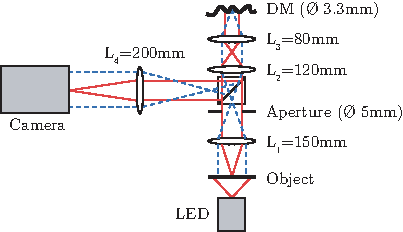
\includegraphics[width=0.50\textwidth]{images/widefield_simple_microscope.pdf}
	\caption{Schematic diagram of the experimental setup, showing a simple microscope complemented with a deformable mirror for aberration correction. Image after~\cite{wide_AOM_loew_freq}.}
	\label{fig:widefield_simple_microscope}
\end{figure}

The presented method uses low spatial frequency content of the image as the optimization metric. The aberration is represented in terms of so called Lukosz modes. Like Zernike polynomials, the Lukosz functions are each expressed as the product of a radial polynomial and an azimuthal function. The presented technique is based on modeling the effects of aberrations on the imaging of low spatial frequencies, which Lukosz modes are are found to be ideal for.

\noindent By modeling the aberration $\Phi(r)$ as a series of $N$ Lukosz modes $L_i(r,\phi)$ with coefficients $a_i$~\cite{wide_Lukosz_Modes}:
\begin{align}
	\Phi(r) = \sum_{i=4}^{N+3}{a_i L_i(r,\phi)},
	\label{eq:aberration_expansion_Lukosz}
\end{align}
they develop the optimization metric $g$ as the sum of a range of low frequencies. It is related to the coefficients of the aberration expansion, $a_i$ by the Lorentzian function~\cite{wide_AOM_loew_freq}
\begin{align}
	g(a_i) \approx \frac{1}{q_0 + q_1 \sum_{i=4}^{N+3}{a_i^2}}
	\label{eq:aberration_metric}
\end{align}
where the piston, tip and tilt modes ($i = 1,2,3$ respectively) have been omitted and $q_0$ and $q_1$ are both positive quantities in the frequency range of interest. The aberration correction process is then performed as the maximization of $g(a_i)$. Because of this particular aberration expansion and  optimization metric, the function $g(a_i)$ shows a paraboloidal maximum that permits the use of simple maximization algorithms. Furthermore, it is shown that the optimization can be performed as a sequence of independent maximizations for each aberration coefficient. 

\begin{figure}[tbh]
			\centering
			\begin{subfigure}[b]{0.8\textwidth}
							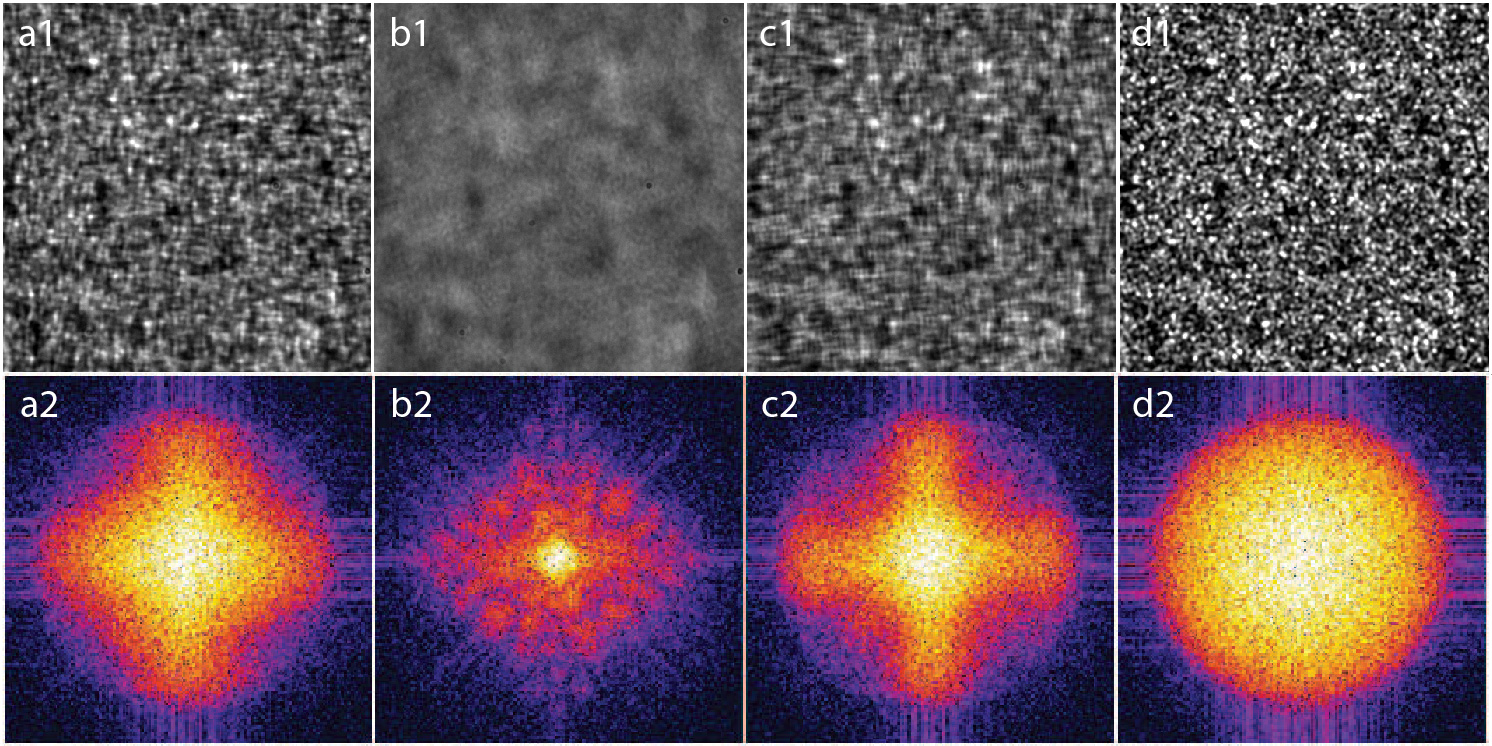
\includegraphics[width=\textwidth]{images/wide_parabolic_opti_images}
							\label{fig:para_opt_images}
			\end{subfigure}
			\begin{subfigure}[b]{0.8\textwidth}
							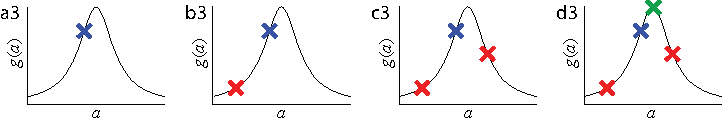
\includegraphics[width=\textwidth]{images/wide_parabolic_opti_graphs}
							\label{fig:para_opt_graphs}
			\end{subfigure}								
			\caption{Correction of a single Lukosz aberration mode (astigmatism, i = 5) for a scatterer specimen and using low spatial frequencies. The first row shows the raw images of the specimen and the second row contains the corresponding spectral densities. The third row illustrates schematically the sampling of the Lorentzian curve used in the optimization calculation. (a1-a3) correspond to an arbitrary initial aberration of magnitude, (b1-b3) have an additional negative bias while (c1-c3) have an additional positive bias of equal magnitude. (d1- d3) show the corrected image calculated with the parabolic minimizationn. Image after~\cite{wide_AOM_loew_freq}.}
	\label{fig:para_opt}
\end{figure} 

The correction process is shown in Figure~\ref{fig:para_opt} for the correction of a single Lukosz mode using a scatterer specimen. Using the deformable mirror (DM), an initial aberration $a_i$ is applied and an image is recorded. The Fourier transform and spectral density of the image are then calculated and the appropriate range of frequency components are summed, giving the metric measurements $g_0$. The same procedure is repeated with both negative and positive aberrations~(i.e. stronger and weaker aberrations), resulting in the metric measurements $g_-$ and  $g_+$. Due to the paraboilc maximum of \eqref{eq:aberration_metric}, the value of $a_i$ that minimizes $g$ can be calculated from as little as three measurements of $g(a_i)$. The optimum correction aberration can then estimated by parabolic minimization as~\cite{wide_parabolic_optimization}:
\begin{align}
	a_\text{corr} = \frac{b(g_+ - g_-)}{2g_+ - 4g_0 + 2g_-}
\end{align}
and is then applied to the DM. To correct multiple modes, each modal coefficient is measured in the same manner before the full correction aberration containing all modes is applied. While this technique is based only on low spatial frequencies, it is shown that both low and high frequency components can be effectively corrected. In all the cases investigated, a Strehl ratio greater than 0.8, close to the diffraction limit, was obtained. This indicates that, when aberration statistics are unknown, choosing small spatial frequencies for an initial correction is a reasonable strategy. If further correction is required,they can be performed using a larger range of frequencies. \emph{Debarre et al.} conclude that this correction scheme is largely independent of the object structure and propose that this approach also to be valid for coherent or partially coherent systems.


%------------------------------------------------------------------------------
\subsubsection{Structured Illumination Microscopy}
\label{sec:StructuredIlluminationMicroscopy}

It is often desired for biological samples to produce clear images of focal planes deep within a thick sample (i.e. optical sectioning) and common techniques include point-scanning techniques such as confocal or multiphoton techniques which are described in Section~\ref{sec:PointScanningMicroscopes}. 

%TODO
Widefield techniques such as Structured Illumination (SI) microscopy can also provide optical sectioning. However, there the sectioning is realized using a standard microscopes, an incoherent light source and without the need for a scanning mechanism. For SI microscopy, a grid is imaged into the specimen to produce a one-dimensional sinusoidal excitation pattern in the focal plane. The resulting sinusoidal fluorescence image, consisting of both in- focus and out-of-focus fluorescence emission, is then normally recorded. Several images are taken, each corresponding to a different grid position equivalent to three different phase shifts of the grating. The grid pattern only appears in the focal plane while it is blurred in the out of focus regions. Hence, it is possible to extract an optical section from the spatially modulated component of the images via a simple calculation.

Based on the SI microscopy technique presented by \emph{Neil et al.} in 2005~\cite{wide_structured_illu_principle} as well as their earlier work on indirect wavefront sensing using a conventional microscope~\cite{wide_AOM_loew_freq} in 2007~(described in the previous section) \emph{Debarre et al.} combined both techniques in 2008 and proposed an AO scheme for use in SI microscopy~\cite{wide_AOM_structured_illu}.  

\begin{figure}
	\centering
		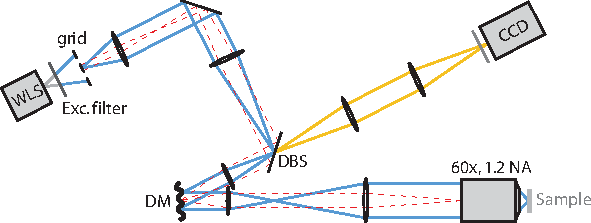
\includegraphics[width=0.75\textwidth]{images/wide_structured_illumination.pdf}
	\caption{Experimental setup for structured illumination microscopy with 
aberration correction. WLS~-~white light source, DM~-~deformable mirror, DBS
~-~dichroic beamsplitter. The blue rays mark the illumination path; the 
detection path is shown in yellow. Image after~\cite{wide_AOM_structured_illu}
.}
	\label{fig:wide_structured_illumination}
\end{figure}

They again present a sensorless wavefront detection scheme, which is shown in Fig.~\ref{fig:wide_structured_illumination}. The method to obtain the aberration correction is similar to the one presented and explained in the previous section. 
The authors derive an inner product from a mathematical model of the imaging process, followed by an orthogonalization process applied to a set of Zernike polynomials. Based on that, a general method providing an optimal aberration expansion for the chosen optimization metric is presented. This process yields  information about the effects of different aberration modes in of the SI microscope. \emph{Debarre et al.} show that the image quality mainly depends on the imaging efficiency spatial frequency of the illumination pattern. This imaging efficiency is affected much more by some aberration modes~(called grid modes) than by others~(called non-grid modes) . Grid modes have a significant influence on the intensity of the sectioned image, whereas non-grid modes have comparatively little effect. The non-grid modes do however affect the resolution. 

The results of the implemented AO scheme is shown in Fig.~\ref{fig:structured_light_correction} for aberration correction on a fluorescent mouse intestine. The image contrast and sharpness improvement is clearly visible in image~\ref{fig:SI_corrected} compared to the uncorrected image in \ref{fig:SI_uncorrected}. As a result of the aberration correction, and as shown in Fig.~\ref{fig:SI_scan}, the contrast of small sample features (blue arrows) is better defined after (red solid line) rather than before (black dotted line) correction. 

\begin{figure}[tbh]
        \centering
        \begin{subfigure}[b]{0.25\textwidth}
                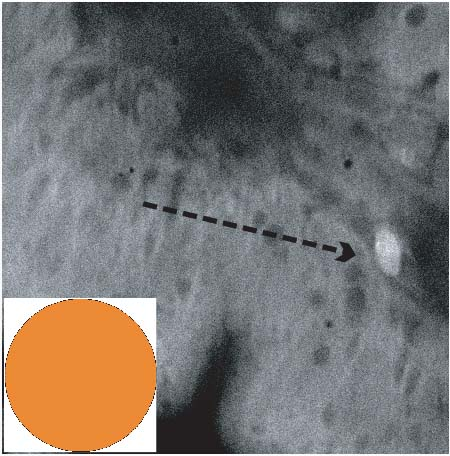
\includegraphics[width=\textwidth]{images/structured_illumination_uncorrected}
                \caption{Uncorrected.}
                \label{fig:SI_uncorrected}
        \end{subfigure}
        \begin{subfigure}[b]{0.25\textwidth}
                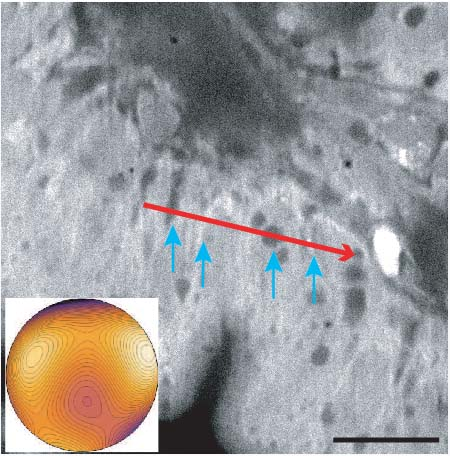
\includegraphics[width=\textwidth]{images/structured_illumination_corrected}
                \caption{Corrected.}
                \label{fig:SI_corrected}
        \end{subfigure}
        \begin{subfigure}[b]{0.25\textwidth}
                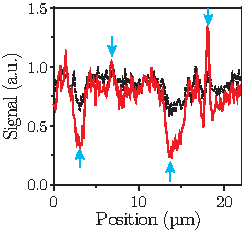
\includegraphics[width=\textwidth]{images/structured_illumination_scan}
                \caption{Line Scan.}
                \label{fig:SI_scan}
        \end{subfigure}
								
        \caption{Aberration correction in structured illumination microscopy. 
A fluorescent mouse intestine sample was imaged (a) without (b) with 
aberration correction with inserts showing the phase induced by the 
deformable mirror. (c) Profile along the lines drawn on the images, both 
profiles normalized so that their mean value is identical. As a result of the 
resolution improvement, the contrast of small sample features (blue arrows) 
is better defined after (red solid line) rather than before (black dotted 
line) correction. The imaging depth was approximately $\unit[10]{\upmu m}$, 
sacle bar size $\unit[10]{\upmu m}$. Image after~\cite{wide_AOM_structured_illu}
.}
\label{fig:structured_light_correction}
\end{figure} 

The authors also explain an additional benefit of aberration correction for structured illumination microscopy. That the adaptive element can also be used to improve the rejection of the out-of-focus fluorescence. When imaging thick specimen, noise fluctuations in the fluorescence signal between the three successive widefield images obtained for the maximization process result in a large out-of-focus background in the calculated sectioned images. Since this background arises from fluorescence generated outside the focal plane, it is not  sensitive to the presence of aberrations. By applying large aberrations in a number of grid modes, the grid pattern is suppressed and only the out-of-focus noise can be measured. By subtracting this aberrated image from the original sectioned image, the fluorescent background can be efficiently removed, leading to greatly improved contrast of the in-focus structures.

The aberrations can also change significantly with depth and hence using the same correction for different depths can result in a degradation of the image quality.  The correction can however be adapted for different imaging depths in the sample. This permits improvement of the image quality throughout an axially extended sample.
It is furthermore possible to determined the appropriate modes once and use the same scheme for any specimen, as the scheme is mostly independent of the object structure. Alternatively, if one wants to correct for local variations in aberrations the image could be formed from several sub-images for which independent aberration correction would be performed.

%TODO is this technique applied in Point Scanning Techniques? 
In conclusion, the authors present a sophisticated, easy to implement and highly versatile AOM scheme which allows for aberration correction induced by the optical system, the specimen or the focus depth. While the presented scheme uses a widefield microscope, \emph{Debarre et al.} are also optimistic that similar AO methods based on indirect, image based aberration detection can be applied to point-scanning methods. 


%------------------------------------------------------------------------------
\subsection{Point Scanning Microscopes}
\label{sec:PointScanningMicroscopes}

Just as with the widefield techniques, adaptive optics quickly found its way into point scanning techniques to improve the image and signal quality. 

Scanning methods are useful for imaging biological specimens, since they can provide high resolution imaging in three-dimensions. Illumination is  usually provided by a laser that is focused into the sample. The light emitted or reflected from the specimen is collected, usually through the same objective lens, and its intensity is measured by a detector. Since this only provides information about the intensity at a single spot, focal point is then scanned through the specimen and point-by-point the image is acquired. 

%ToDo - check what we will actually describe and write short intro for that here...
Several other point scanning microscope modalities have been introduced, including Two-Photon Excitation Fuorescence (TPEF) microscopy, second harmonic generation (SHG) and third harmonic generation (THG) microscopy, and coherent anti-Stokes Raman (CARS) microscopy.

- using a fluorescence microscope, the smaller FWHM, provided by the optimized DMM, will increase the excitation intensity leading to a higher fluorescent signal for the same laser beam input power

3D adaptive optics in a light sheet microscope~\cite{scan_lightSheet}

%------------------------------------------------------------------------------
-
\subsubsection{Confocal Microscopes}
\label{sec:ConfocalMicroscopes}

The most common example of this type is the confocal microscope, which can be 
operated in reflection or fluorescence mode. Three-dimensional resolution is 
achieved by the placement of a pinhole in front of the photodetector. In a 
reflection mode confocal microscope, the illumination is scattered by objects 
not only in the focal region, but throughout the focusing cone. In 
fluorescence mode, emission is generated in the focus but also in out-of-
focus regions. The pinhole ensures that mainly light from the focal region 
falls upon the detector and light from out-of-focus planes is obscured. It is 
critical in the confocal microscope that both the illumination and detection 
paths are diffraction limited. This ensures that i) the illuminating focal 
spot is as small as possible, and ii) that the focus is perfectly imaged on 
to the detector pinhole. Therefore, in an adaptive confocal microscope, 
aberration correction must be included in both paths. This dual pass adaptive 
system can usually be implemented using a single deformable mirror, if the 
path length aberrations are the same for both the illumination and the 
emission light. This is the case if there is no significant dispersion in the 
specimen or chromatic aberration in the optics.

A pinhole is not required to obtain three-dimensional resolution, so most 
TPEF microscopes use large area detectors to maximise signal collection. 
Although they rely upon other physical processes, non-linear imaging 
modalities such as SHG, THG and CARS exhibit similar resolution properties. 
When using large area detectors, the fidelity of imaging in the detection 
path is unimportant so the effects of any aberrations in this path are 
negated. It follows that single pass adaptive optics is appropriate for these 
microscopes as aberration correction need only be implemented in the 
illumination path.

Adaptive optics systems have been successfully combined with several point-
scanning microscope systems including confocal,13 TPEF,6, 14, 15 harmonic 
generation,16, 17 CARS.18 Example images of aberration correction in an 
adaptive THG microscope are shown in Fig. 10.

\cite{book_confocal}
\cite{scan_CFM}

%------------------------------------------------------------------------------
\subsubsection{Two-Photon Fluorescence Microscopy}
\label{sec:twoPhotonExcitation}

Its intrinsic optical sectioning, larger penetration depth, reduced photo damage as well as other advantages allowed nonlinear microscopy in general, and Two-Photon Fluorescence Microscopy~(TPFM) in particular, to become a very important tool in biological imaging since its first presentation by \emph{Denk at al.} in 1990~\cite{scan_TPFM_principle}.

As with most AO microscopy techniques, both a direct and indirect wavefront sensing scheme can be deployed for the use with TPFM. Indirect sensing was already explained~(section~\ref{sec:IndirectWavefrontSensing}) and presented~(section~\ref{sec:WidefieldMicroscopy} in detail. \emph{Marsh et al.} present the first and fairly simple indirect sensing approach, correcting only for depth induced aberrations as early as 2003~\cite{scan_TPFM_pratical}. Again, based on their earlier works~(\cite{wide_AOM_loew_freq,wide_AOM_structured_illu}), \emph{D\'{e}barre et al.} present another highly sophisticated application of their image based wavefront sensing scheme in 2009~\cite{scan_TPFM_image_based}. Both \emph{Marsh} and \emph{D\'{e}barre} essentially use the standard TPFM setup and the image optimization is very similar to the one presented earlier, we will not describe these methods here again.

\emph{Rueckel et al.} present a wavefront correction method using coherence-gated wavefront sensing~\cite{scan_TPFM_gated_wavefront} which also beyond the scope of this report. This section will therefor describe direct wavefront sensing based on the work presented by \emph{Aviles-Espinosa et al.} in 2011~\cite{scan_TPFM_guide_start}.

%rewrite for use here, good general intro....
The resolution has a high dependence on the point-spread function (psf) of the scanned point source. Additionally, the signal levels in two-photon fluorescence have a strong nonlinear dependence upon the incident light intensity. Thus the ideal is to image the sample by use of a diffraction limited spot. However, refractive-index mismatches between the immersion media of high-NA objectives and the sample, in addition to the usually nonuniform samples themselves, impart aberrations to the wavefront and contribute to a deterioration of the psf. Other sources of aberrations include off-axis transmission through optical components, such as the objective and scan lenses while scanning, and imperfections in the optical elements throughout the optical train. The net effect of specimen induced aberrations is that while reducing the achievable resolution, the necessary laser power to achieve imaging increases with depth which can lead to nonreversible effects in biological samples. It also places greater demands in terms of output power on multiphoton imaging laser sources.

%based on \cite{scan_TPFM_guide_start}
- no need to correct on the collected beam as light is only emitted in focus region
- correcting the excitation beam is a must as this will ensure a better focusing and therefore, a more efficient nonlinear (NL) process
- sensor-less schemes, iterative algorithms are generally used to control a deformable mirror (DM) or a Spatial Light Modulator 
- it has been reported the use of optimized algorithms reduce sample exposure
- still implies that an area of interest within the sample has to be exposed a considerable number of times
- may result in unwanted exposure which is prone to produce photo-bleaching and photo-toxic effects on the sample
- We demonstrate that sample induced aberrations can be measured and corrected, 
- In sensor-based schemes  correction performed by measuring aberrations through a wavefront sensor 
- employing a reference point source called guide star
- Then such information is fed to a DM, in order to restore the image quality.
- information is then fed into an adaptive element and aberration is corrected 
- all explained in detail in \ref{sec:WavefrontSensing}
- guide star has been applied for moderate scattering samples imaged through linear fluorescence microscopy~\cite{wide_fluorescence_guide_star} 
- artificially inserting a small, fixed secondary light source inside the sample 
- allows for a direct measurement of the sample aberrations using a Shack-Hartmann (SH) WFS,
- based on the introduction of beads inside the sample 
- it is prone to cause sample damage, limiting its potential for in vivo imaging studies
- beads are randomly distributed inside the fixed sample, suitable bead placed at the right location must be found in the field of view (FOV) and for each depth to be imaged
- adds complexity to the sample preparation and to the aberration measurement process
- Two-photon excited fluorescence (TPEF) naturally produces a small confined volume which can be used as an incoherent secondary light source
- this point source, authors refer to as "`nonlinear guide-star"' (NL-GS), can be used for single pass measurements of sample and objective aberrations
- uses the fact that two-photon excited fluorescence naturally produces a localized point source inside the sample: the nonlinear guide-star (NL-GS).
- The wavefront emitted from the NL-GS can then be recorded using a Shack-Hartmann sensor.
- Compensation of the recorded sample aberrations is performed by the deformable mirror in a single-step. 
- applied to fixed and in vivo biological samples, showing, in some cases, more than one order of magnitude improvement in the total collected signal intensity.
- measured using a WFS placed at the output port of the NLM microscope
- as the WF is directly expressed in the form of Zernike coefficients, it is possible to shape the adaptive element (DM) in a single step (i.e. without the need of any search algorithm) for correcting the measured aberrations
- so, image quality and contrast can be significantly improved without having to expose the sample for large periods of time
- Consequently photo-bleaching and photo-toxicity are greatly reduced
- it can be applied in vivo, it is simple, noninvasive and requires no additional sample processing (such as the incorporation of fluorescent beads)
- Moreover, the NL-GS can be created at any desired position inside a sample
- has been demonstrated with both, moderate and increased scattering samples.
- For moderate scattering samples, when comparing coupling vs. focusing aberrations, we found that the total signal improvement can be up to 11.66 times 
- For samples with increased scattering correction is moderate but in agreement with other adaptive optics correction schemes

\begin{figure}
	\centering
		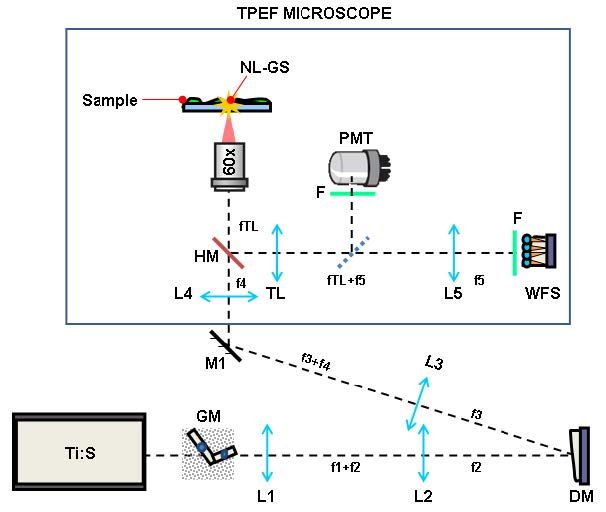
\includegraphics[width=0.75\textwidth]{images/TPFM_guide-star.jpg}
	\caption{check if we really want this...\cite{scan_TPFM_guide_start} Use it...do it yourself and make it nice!!!}
	\label{fig:TPFM_guide-star}
\end{figure}

\cite{scan_TPFM_guide_start}

%------------------------------------------------------------------------------
\subsubsection{Harmonic Generation}
\label{sec:HarmonicGeneration}

\cite{scan_HG_embryos}
\cite{scan_HG_dynamic}


%------------------------------------------------------------------------------
\subsubsection{CARS}
\label{sec:CARS}

\cite{scan_CARS}

%------------------------------------------------------------------------------
\subsubsection{STED}
\label{sec:STED}

\cite{scan_STED}




%%%%%%%%%%%%%%%%%%%%%%%%%%%%%%%%%%%%%%%%%%%%%%%%%%%%%%%%%%%%%%%%%%%%%%%%%%%%%%%
\section{Conclusion \& Future Prospects}
\label{sec:Future}
%%%%%%%%%%%%%%%%%%%%%%%%%%%%%%%%%%%%%%%%%%%%%%%%%%%%%%%%%%%%%%%%%%%%%%%%%%%%%%%

While adaptive optics has been applied in many fields for more than fifteen years, in biological imaging it is still a relatively new system. Since new AO techniques for modern microscopes are just being developed, it will take more time before AO can become a standard component of laboratory microscopes.  

It is important to remark that AO applied to microscopy does not overcome the diffraction limit but rather helps to restore a diffraction limited imaging case. It therefore usually yields in an improvement in both axial and lateral resolution as well as an increase in signal intensity. In other words, AO extends the capabilities of high-resolution or superesolution techniques, especially extending the ability to image deeper into tissue. The advantages of correcting aberrations always depend on the specimen under study and the microscopy technique used. One of the most critical issues in AO applied to microscopy is the accuracy in the sensing process, that is, how we obtain the aberration information from the sample. It seems to be that indirect sensing is the first option in almost all the experiments for AO microscopes. This is because it is easier to implement in microscopy since it only requires a deformable mirror and no point-like emitter is needed. Indirect sensing is however usually slower than direct sensing. 

An important drawback in most AO methods for microscopy is the relatively slow wavefront detection. As long as aberrations don't change quickly or when just considering a small region of a sample, this is not a problem. However, when imaging larger parts of a sample or when trying to image fast processes in live samples, AO techniques are often slow. Thus, it is important to further optimize the current systems or to develop a completely new, faster correction devices~(using multiple correctors being a possible solution). This would extend the ability to correct aberrations in real time and with less exposure of the specimens during the measurement. The slow sensing is also an important drawback for aberration correction in an industrial microscope used in hospitals or biological labs. Thorlabs offers a ready-made adaptive optics system for TPFM~\cite{future_thorlabs} but it also aims at research labs and is not suitable for the end user. Big microscope manufacturers like Zeiss and Leica have not yet presented a single commercial microscope using adaptive optics, even though Zeiss owns a patent on the technology~\cite{future_zeiss_patent}. Furthermore, AO methods have not been implemented in techniques such as STORM and PALM yet. First publications in these fields are only a matter of time and are probably due to the young age of the methods, as AO techniques are currently being developed~\cite{future_AOM_PALM_1}. \newline

\noindent It is difficult to give specific advice regarding the choice of the correct adaptive optics system. If measurement speed and photobleaching are a concern, direct sensing should be considered, with the possible downside of a higher complexity and the need for a guide star. If a maximal signal intensity is more important, photobleaching is not a problem and if space, hardware and budget are limited, indirect sensing might be the better choice. It offers a cheap and easy AO implementation if time is not a concern or if suitable optimization algorithms can be developed. In the end, the right choice has to be determined based on the microscopy technique and system constrains. Despite all this, further improvements in the sensing and correction process will certainly further extend the already wide range AO applications in modern microscopes in the future. 

%% Bibliographie %%%%%%%%%%%%%%%%%%%%%%%%%%
\clearpage
\bibliographystyle{myStyle} %bib style created with myBst package
\bibliography{tex/bibo}	%insert name of .bib file

\clearpage

%\setcounter{section}{0}%
%\renewcommand{\thesection}{\Alph{section}}%
%\input{tex/x_appendix.tex}
\end{document}
